\section{Orthogonal projections and Fourier series}

We now reconsider a problem that we briefly encountered, only in the
context of $\R^3$, in Section~\ref{sec:planes}: how to find the
shortest distance between a point and a subspace. The method we used
in Section~\ref{sec:planes} (see
Example~\ref{exa:shortest-distance-plane}) relies on the existence of
normal vectors and does not generalize beyond $\R^3$. The following
proposition gives a much better method for solving this problem,
provided that we have an orthogonal basis of the subspace.

\begin{proposition}{Orthogonal projection onto a subspace}{projection-subspace}
  Let $V$ be an inner product space, and let $W$ be a subspace of
  $V$. Assume $\set{\vect{u}_1,\ldots,\vect{u}_k}$ is an orthogonal
  basis of\/ $W$, and $\vect{v}\in V$ is any vector. Then the
  following vector $\vect{v}'$ is the element of $W$ that is closest
  to $\vect{v}$, i.e., such that $\norm{\vect{v}-\vect{v}'}$ is as
  small as possible.
  \begin{equation*}
    \vect{v}' =
    \frac{\iprod{\vect{v},\vect{u}_1}}{\iprod{\vect{u}_1,\vect{u}_1}}\,\vect{u}_1
    + \frac{\iprod{\vect{v},\vect{u}_2}}{\iprod{\vect{u}_2,\vect{u}_2}}\,\vect{u}_2
    + \ldots
    + \frac{\iprod{\vect{v},\vect{u}_k}}{\iprod{\vect{u}_k,\vect{u}_k}}\,\vect{u}_k.
  \end{equation*}
  Moreover, the vector $\vect{v}-\vect{v}'$ is orthogonal to $W$.
  \begin{center}
    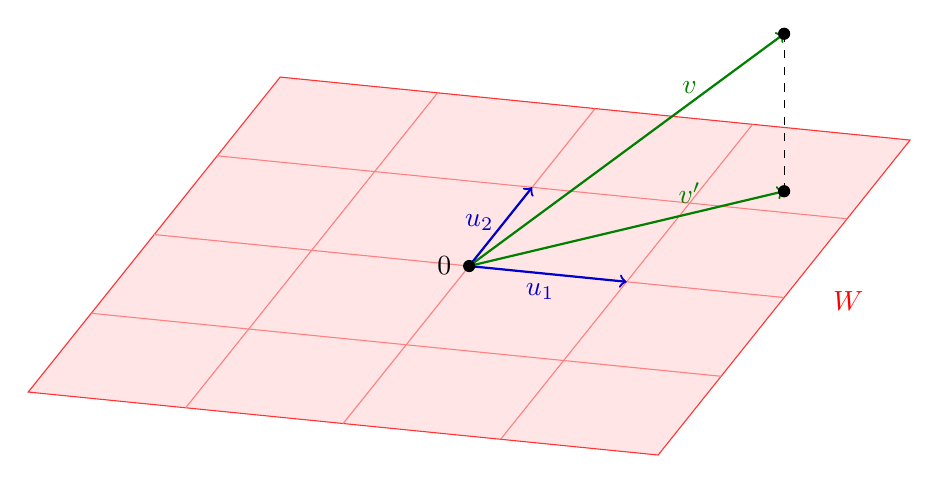
\begin{tikzpicture}[x={(1cm,-0.1cm)},y={(0.4cm,0.5cm)},z={(0cm,1cm)}]
      \filldraw[draw=red!80,fill=red!10](-4,-4,0) -- (4,-4,0) -- (4,4,0) -- (-4,4,0) -- cycle;
      \path[red] (4.5,0,0) node[right] {$W$};
      \draw[thin,red!50] (-2,-4,0) -- (-2,4,0);
      \draw[thin,red!50] (0,-4,0) -- (0,4,0);
      \draw[thin,red!50] (2,-4,0) -- (2,4,0);
      \draw[thin,red!50] (-4,-2,0) -- (4,-2,0);
      \draw[thin,red!50] (-4,0,0) -- (4,0,0);
      \draw[thin,red!50] (-4,2,0) -- (4,2,0);
      \draw[->,thick,blue!80!black](0,0,0) -- node[below, pos=0.45]{$\vect{u}_1$} (2,0,0);
      \draw[->,thick,blue!80!black](0,0,0) -- node[left, pos=0.55]{$\vect{u}_2$} (0,2,0);
      \draw[->,thick,green!50!black](0,0,0) -- node[above, pos=0.7] {$\vect{v}$} (3,2.5,2);
      \draw[->,thick,green!50!black](0,0,0) -- node[above, pos=0.7] {$\vect{v}'$} (3,2.5,0);
      \draw[dashed](3,2.5,0) -- (3,2.5,2);
      \fill (0,0,0) circle [radius=2.2pt] node [left=3pt] {$\vect{0}$};
      \fill (3,2.5,2) circle [radius=2.2pt];
      \fill (3,2.5,0) circle [radius=2.2pt];
    \end{tikzpicture}
  \end{center}
  The vector $\vect{v}'$ is called the \textbf{orthogonal projection
    of $\vect{v}$ onto $W$}%
  \index{orthogonal projection!onto subspace}%
  \index{projection!onto subspace}. We also say that $\vect{v}'$ is
  the \textbf{best approximation}%
  \index{approximation} of $\vect{v}$ in $W$.
\end{proposition}

\begin{proof}
  Since $\set{\vect{u}_1,\ldots,\vect{u}_k}$ is a basis of $W$, every
  vector $\vect{w}\in W$ is of the form
  $\vect{w} = x_1\vect{u}_1 + \ldots + x_k\vect{u}_k$, where
  $x_1,\ldots,x_k\in\R$. We have
  \begin{eqnarray*}
    \norm{\vect{v}-\vect{w}}^2
    &=& \iprod{\vect{v}-\vect{w}, \vect{v}-\vect{w}} \\
    &=& \iprod{\vect{v}, \vect{v}} - 2\iprod{\vect{v},\vect{w}} + \iprod{\vect{w},\vect{w}} \\
    &=& \iprod{\vect{v}, \vect{v}} - 2\iprod{\vect{v},x_1\vect{u}_1 + \ldots + x_k\vect{u}_k} + \iprod{x_1\vect{u}_1 + \ldots + x_k\vect{u}_k, x_1\vect{u}_1 + \ldots + x_k\vect{u}_k} \\
    &=& \iprod{\vect{v}, \vect{v}} - 2x_1\iprod{\vect{v},\vect{u}_1} - \ldots - 2x_k\iprod{\vect{v},\vect{u}_k} + x_1^2\iprod{\vect{u}_1, \vect{u}_1} + \ldots + x_k^2\iprod{\vect{u}_k, \vect{u}_k} \\
    &=& \iprod{\vect{v}, \vect{v}} + (x_1^2\iprod{\vect{u}_1, \vect{u}_1} - 2x_1\iprod{\vect{v},\vect{u}_1}) + \ldots + (x_k^2\iprod{\vect{u}_k, \vect{u}_k} - 2x_k\iprod{\vect{v},\vect{u}_k}).
  \end{eqnarray*}
  Here, in the second-to-last step, we have used the fact that
  $\iprod{\vect{u}_i,\vect{u}_j}=0$ when $i\neq j$, i.e., the
  orthogonality of $\vect{u}_1,\ldots,\vect{u}_k$.  Therefore, the
  expression $\norm{\vect{v}-\vect{w}}^2$ is minimized when each of the
  expressions
  \begin{equation}\label{eqn:projection-subspace}
    x_1^2\iprod{\vect{u}_1, \vect{u}_1} - 2x_1\iprod{\vect{v},\vect{u}_1}, \qquad
    \ldots,\qquad
    x_k^2\iprod{\vect{u}_k, \vect{u}_k} - 2x_k\iprod{\vect{v},\vect{u}_k}
  \end{equation}
  takes its minimum. By the laws of calculus, the minimum of a
  function of the form $f(x)=ax^2-2bx$ occurs when $f'(x)=2ax-2b=0$,
  i.e., when $x=\frac{b}{a}$. Applying this reasoning to each of the
  $k$ expressions in {\eqref{eqn:projection-subspace}}, we find that the
  minimum occurs when
  \begin{equation*}
    x_1 = \frac{\iprod{\vect{v},\vect{u}_1}}{\iprod{\vect{u}_1,\vect{u}_1}},\quad
    \ldots,\quad
    x_k = \frac{\iprod{\vect{v},\vect{u}_k}}{\iprod{\vect{u}_k,\vect{u}_k}},
  \end{equation*}
  i.e., when
  \begin{equation*}
    \vect{w} =
    \frac{\iprod{\vect{v},\vect{u}_1}}{\iprod{\vect{u}_1,\vect{u}_1}}\,\vect{u}_1
    + \frac{\iprod{\vect{v},\vect{u}_2}}{\iprod{\vect{u}_2,\vect{u}_2}}\,\vect{u}_2
    + \ldots
    + \frac{\iprod{\vect{v},\vect{u}_k}}{\iprod{\vect{u}_k,\vect{u}_k}}\,\vect{u}_k.
  \end{equation*}
  This is what had to be shown. Finally, to show that
  $\vect{v}-\vect{v}'$ is orthogonal to $W$, it suffices to show that
  $\vect{v}-\vect{v}'$ is orthogonal to each basis vector
  $\vect{u}_1,\ldots,\vect{u}_k$ of $W$. We show this by direct calculation.
  Consider $i\in\set{1,\ldots,k}$. First note that
  \begin{eqnarray*}
    \iprod{\vect{v}',\vect{u}_i}
    &=& \bigiprod{\paren{
        \frac{\iprod{\vect{v},\vect{u}_1}}{\iprod{\vect{u}_1,\vect{u}_1}}\,\vect{u}_1
        + \ldots
        + \frac{\iprod{\vect{v},\vect{u}_k}}{\iprod{\vect{u}_k,\vect{u}_k}}\,\vect{u}_k}
        ,\vect{u}_i}\\
    &=&
        \frac{\iprod{\vect{v},\vect{u}_1}}{\iprod{\vect{u}_1,\vect{u}_1}}\,\iprod{\vect{u}_1,\vect{u}_i}
        + \ldots
        + \frac{\iprod{\vect{v},\vect{u}_k}}{\iprod{\vect{u}_k,\vect{u}_k}}\,\iprod{\vect{u}_k,\vect{u}_i}
    \\
    &=& \frac{\iprod{\vect{v},\vect{u}_i}}{\iprod{\vect{u}_i,\vect{u}_i}}\,\iprod{\vect{u}_i,\vect{u}_i}\\
    &=& \iprod{\vect{v},\vect{u}_i}.
  \end{eqnarray*}
  Therefore,
  $\iprod{\vect{v}-\vect{v}',\vect{u}_i} = \iprod{\vect{v},\vect{u}_i}
  - \iprod{\vect{v}',\vect{u}_i} = 0$, and $\vect{v}-\vect{v}'$ is
  orthogonal to $\vect{u}_i$, as desired.
\end{proof}

\begin{example}{Orthogonal projection onto a subspace}{projection-subspace}
  Consider $\R^4$ with the usual dot product. Let
  $W=\sspan\set{\vect{u}_1,\vect{u}_2}$, where
  \begin{equation*}
    \vect{u}_1 = \begin{mymatrix}{r} 1 \\ 1 \\ 2 \\ 0 \end{mymatrix}, \quad
    \vect{u}_2 = \begin{mymatrix}{r} -1 \\ -1 \\ 1 \\ 3 \end{mymatrix}.
  \end{equation*}
  Note that $\vect{u}_1$ and $\vect{u}_2$ are orthogonal. Let
  \begin{equation*}
    \vect{v} = \begin{mymatrix}{r} 1 \\ 2 \\ 3 \\ 4 \end{mymatrix}.
  \end{equation*}
  Find the best approximation of $\vect{v}$ in $W$.
\end{example}

\begin{solution}
  We calculate $\iprod{\vect{v},\vect{u}_1}=9$,
  $\iprod{\vect{u}_1,\vect{u}_1}=6$, $\iprod{\vect{v},\vect{u}_2}=12$,
  and $\iprod{\vect{u}_2,\vect{u}_2}=12$. Therefore, by
    Proposition~\ref{prop:projection-subspace}, the desired vector is
  \begin{equation*}
    \vect{v}'
    ~=~ \frac{\iprod{\vect{v},\vect{u}_1}}{\iprod{\vect{u}_1,\vect{u}_1}}\,\vect{u}_1
    + \frac{\iprod{\vect{v},\vect{u}_2}}{\iprod{\vect{u}_2,\vect{u}_2}}\,\vect{u}_2
    ~=~ \frac{9}{6} \begin{mymatrix}{r} 1 \\ 1 \\ 2 \\ 0 \end{mymatrix}
    + \frac{12}{12} \begin{mymatrix}{r} -1 \\ -1 \\ 1 \\ 3 \end{mymatrix}
    ~=~ \begin{mymatrix}{c} 1/2 \\ 1/2 \\ 4 \\ 3 \end{mymatrix}.
  \end{equation*}
\end{solution}

Note how straightforward the calculations in this example are. All we
had to do is calculate a few inner products. It is not even necessary
to solve a system of equations. Such is the power of orthogonal bases.

The next example shows that we can use exactly the same method to find
approximations%
\index{approximation!of functions} of functions.

\begin{example}{Approximating a function by a polynomial}{projection-subspace-polynomial}
  Let $V=C[-1,1]$ be the vector space of continuous functions, with the
  inner product given by
  \begin{equation*}
    \iprod{f,g} = \int_{-1}^{1} f(x)g(x)\,dx.
  \end{equation*}
  Consider the function $f\in V$ given by
  \begin{equation*}
    f(x)
    ~=~ 1-\abs{x}
    ~=~ \begin{cases}
      1+x & \text{if $x<0$,} \\
      1-x & \text{if $x\geq 0$.}
    \end{cases}
  \end{equation*}
  Find the closest approximation to $f$ by a polynomial of degree at
  most 2. Graph both $f$ and the approximating polynomial.
\end{example}

\begin{solution}
  Let $W=\sspan\set{1,x,x^2}$ be the subspace of $V$ consisting of
  polynomials of degree at most 2. What we are looking for is an
  element $g\in W$ such that $\norm{f-g}$ is as small as possible.  We
  can solve this problem using
  Proposition~\ref{prop:projection-subspace}.

  First we need an orthogonal basis for $W$. We found such an
  orthogonal basis in Example~\ref{exa:legendre-polynomials}, namely
  the Legendre polynomials $p_0(x) = 1$, $p_1(x) = x$, and
  $p_2(x) = x^2-\frac{1}{3}$.  By
  Proposition~\ref{prop:projection-subspace}, the desired
  approximation $g\in W$ is given by:
  \begin{equation*}
    g
    ~=~
    \frac{\iprod{f,p_0}}{\iprod{p_0,p_0}}\,p_0
    + \frac{\iprod{f,p_1}}{\iprod{p_1,p_1}}\,p_1
    + \frac{\iprod{f,p_2}}{\iprod{p_2,p_2}}\,p_2.
  \end{equation*}
  We already computed the inner products $\iprod{p_0,p_0}=2$,
  $\iprod{p_1,p_1}=\frac{2}{3}$, and $\iprod{p_2,p_2}=\frac{8}{45}$ in
  Example~\ref{exa:legendre-polynomials}. We calculate the remaining
  inner products:
  \begin{eqnarray*}
    \iprod{f,p_0}
    &=& \int_{-1}^{1} f(x)\cdot 1\,dx
        ~=~ \int_{-1}^{0} (1+x)\cdot 1\,dx
        +   \int_{0}^{1} (1-x)\cdot 1\,dx
        ~=~ \frac{1}{2} + \frac{1}{2}
        ~=~ 1, \\
    \iprod{f,p_1}
    &=& \int_{-1}^{1} f(x)\cdot x\,\,dx
        ~=~ \int_{-1}^{0} (1+x)\cdot x\,\,dx
        +   \int_{0}^{1} (1-x)\cdot x\,\,dx
        ~=~ -\frac{1}{6} + \frac{1}{6}
        ~=~ 0, \\
    \iprod{f,p_2}
    &=& \int_{-1}^{1} f(x)\cdot (x^2-\frac{1}{3}) dx \\
    &=& \int_{-1}^{0} (1+x)\cdot (x^2-\frac{1}{3})\,dx
        +   \int_{0}^{1} (1-x)\cdot (x^2-\frac{1}{3})\,dx
        ~=~ - \frac{1}{12} - \frac{1}{12}
        ~=~ -\frac{1}{6}. \\
  \end{eqnarray*}
  Therefore,
  \begin{eqnarray*}
    g
    &=&
    \frac{\iprod{f,p_0}}{\iprod{p_0,p_0}}\,p_0
        + \frac{\iprod{f,p_1}}{\iprod{p_1,p_1}}\,p_1
        + \frac{\iprod{f,p_2}}{\iprod{p_2,p_2}}\,p_2
    \\
    &=& \frac{1}{2}\,p_0
        + \frac{0}{2/3}\,p_1
        - \frac{1/6}{8/45}\,p_2
    \\
    &=& \frac{1}{2} 
        - \frac{15}{16}(x^2-\frac{1}{3})
    \\
    &=& \frac{13}{16} - \frac{15}{16}x^2.
  \end{eqnarray*}
  The following graph shows the function $f(x)$ as well as the
  polynomial $g(x)$:
  \begin{center}
    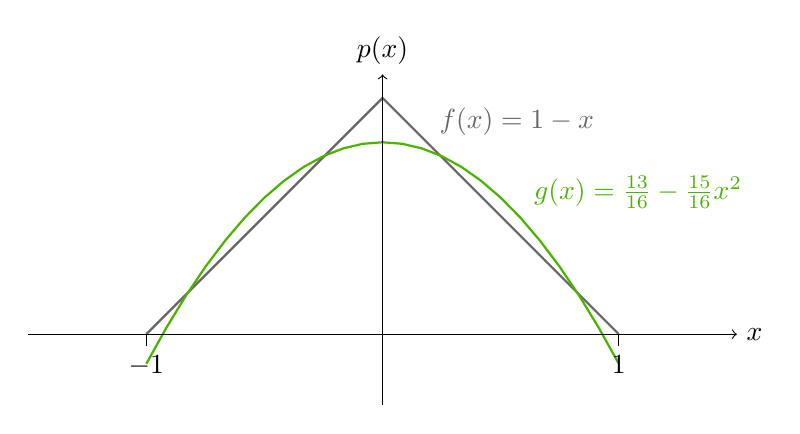
\begin{tikzpicture}[domain=-1:1, scale=3, samples=25]
      \def\fA#1{1}
      \def\fC#1{(abs((#1)^2)-1/3)}
      \definecolor{my-gray}{rgb}{0.4,0.4,0.4}
      \definecolor{my-green}{rgb}{0.3,0.7,0}
      \draw[thick,color=my-gray] (-1,0) -- (0,1) -- (1,0);
      \draw[thick,color=my-green] plot (\x,{0.5*\fA{\x} - 0.9375*\fC{\x}});
      \path[color=my-green] (0.6,0.6) node[right]{$g(x)= \frac{13}{16} - \frac{15}{16}x^2$};
      \path[color=my-gray] (0.2,0.9) node[right]{$f(x) = 1-\abs{x}$};
      \draw[->] (-1.5,0) -- (1.5,0) node[right] {$x$};
      \draw[->] (0,-0.3) -- (0,1.1) node[above] {$p(x)$};
      \draw (1,0) -- (1,-0.05) node[below] {$1$};
      \draw (-1,0) -- (-1,-0.05) node[below] {$-1$};
    \end{tikzpicture}
  \end{center}
\end{solution}

When approximating a function $f$ by a polynomial, as in the last
example, there is no need to stop with polynomials of degree 2. We can
also ask what is the best approximation%
\index{approximation!of functions} of $f$ by a polynomial of
degree 3, of degree 4, of degree 5, and so on. By increasing the
degree of the polynomials, we get better and better approximations to
$f$. This leads us to the concept of a generalized Fourier series.

\begin{definition}{Generalized Fourier series}{generalized-fourier-series}
  Let $V$ be an inner product space and let
  $\set{\vect{u}_1,\vect{u}_2,\vect{u}_3,\ldots}$ be an infinite
  orthogonal set of vectors.  Let $\vect{v}\in V$. The
  \textbf{generalized Fourier series}%
  \index{generalized Fourier series}%
  \index{Fourier series!generalized}%
  \index{series!Fourier series} of $\vect{v}$ (with respect to
  $\vect{u}_1,\vect{u}_2,\vect{u}_3,\ldots$) consists of the following
  sequence of vectors:
  \begin{eqnarray*}
    \vect{v}_1
    &=& \frac{\iprod{\vect{v},\vect{u}_1}}{\iprod{\vect{u}_1,\vect{u}_1}}\,\vect{u}_1, \\
    \vect{v}_2
    &=& \frac{\iprod{\vect{v},\vect{u}_1}}{\iprod{\vect{u}_1,\vect{u}_1}}\,\vect{u}_1
        + \frac{\iprod{\vect{v},\vect{u}_2}}{\iprod{\vect{u}_2,\vect{u}_2}}\,\vect{u}_2, \\
    \vect{v}_3
    &=& \frac{\iprod{\vect{v},\vect{u}_1}}{\iprod{\vect{u}_1,\vect{u}_1}}\,\vect{u}_1
        + \frac{\iprod{\vect{v},\vect{u}_2}}{\iprod{\vect{u}_2,\vect{u}_2}}\,\vect{u}_2
        + \frac{\iprod{\vect{v},\vect{u}_3}}{\iprod{\vect{u}_3,\vect{u}_3}}\,\vect{u}_3, \\
    \vect{v}_4
    &=& \frac{\iprod{\vect{v},\vect{u}_1}}{\iprod{\vect{u}_1,\vect{u}_1}}\,\vect{u}_1
        + \frac{\iprod{\vect{v},\vect{u}_2}}{\iprod{\vect{u}_2,\vect{u}_2}}\,\vect{u}_2
        + \frac{\iprod{\vect{v},\vect{u}_3}}{\iprod{\vect{u}_3,\vect{u}_3}}\,\vect{u}_3
        + \frac{\iprod{\vect{v},\vect{u}_4}}{\iprod{\vect{u}_4,\vect{u}_4}}\,\vect{u}_4, \\
    &\vdots        &
  \end{eqnarray*}
  The vectors $\vect{v}_i$ are also called \textbf{generalized Fourier
    approximations}%
  \index{Fourier approximation}%
  \index{approximation!Fourier} of $\vect{v}$.
\end{definition}

By Proposition~\ref{prop:projection-subspace}, we know that each
$\vect{v}_i$ is the best approximation of $\vect{v}$ in the subspace
$\sspan\set{\vect{u}_1,\ldots,\vect{u}_i}$. In particular,
$\norm{\vect{v}-\vect{v}_{i+1}} \leq \norm{\vect{v}-\vect{v}_i}$, so
each $\vect{v}_i$ is potentially a better approximation of $\vect{v}$
than the previous one. In a course on analysis%
\footnote{``Algebra'' is the name for those subjects where all sums
  are finite. This includes, for example, linear algebra and abstract
  algebra. ``Analysis'' is the name for those subjects where sums are
  potentially infinite (and may or may not converge). This includes,
  for example, calculus, complex analysis, and functional analysis.},
you will learn that in many situations, the sequence
$\vect{v}_1,\vect{v}_2,\vect{v}_3,\ldots$ can be shown to converge to
$\vect{v}$.

\begin{example}{Generalized Fourier series}{generalized-fourier-series}
  Proceeding as in Example~\ref{exa:projection-subspace-polynomial},
  find the generalized Fourier approximations of $f(x)=1-\abs{x}$ up
  to degree 8.
\end{example}

\begin{solution}
  We use the Legendre polynomials $p_0,\ldots,p_8$ from
  Section~\ref{sec:gram-schmidt} and calculate the relevant inner
  products, each of which requires solving an integral. As these
  integrals get a bit complicated, it is best to use a computer
  algebra system to compute them.
  \begin{equation*}
    \def\arraystretch{1.4}
    \begin{array}{rcl}
      \iprod{f,p_0} &=& 1, \\
      \iprod{f,p_1} &=& 0, \\
      \iprod{f,p_2} &=& -\frac{1}{6}, \\
      \iprod{f,p_3} &=& 0, \\
      \iprod{f,p_4} &=& \frac{1}{105}, \\
      \iprod{f,p_5} &=& 0, \\
      \iprod{f,p_6} &=& -\frac{1}{924}, \\
      \iprod{f,p_7} &=& 0, \\
      \iprod{f,p_8} &=& \frac{1}{6435}, \\
    \end{array}
    \quad
    \begin{array}{rcl}
      \iprod{p_0,p_0} &=& 2, \\
      \iprod{p_1,p_1} &=& \frac{2}{3}, \\
      \iprod{p_2,p_2} &=& \frac{8}{45}, \\
      \iprod{p_3,p_3} &=& \frac{8}{175}, \\
      \iprod{p_4,p_4} &=& \frac{128}{11025}, \\
      \iprod{p_5,p_5} &=& \frac{128}{43659}, \\
      \iprod{p_6,p_6} &=& \frac{512}{693693}, \\
      \iprod{p_7,p_7} &=& \frac{512}{2760615}, \\
      \iprod{p_8,p_8} &=& \frac{32768}{703956825}. \\
    \end{array}
  \end{equation*}
  We therefore have the following approximations:
  \begin{eqnarray*}
    f_0 &=& f_1 ~~=~~
            \frac{1}{2}\,p_0,
    \\
    f_2 &=& f_3 ~~=~~
            \frac{1}{2}\,p_0
            - \frac{15}{16}\,p_2,
    \\
    f_4 &=& f_5 ~~=~~
            \frac{1}{2}\,p_0
            - \frac{15}{16}\,p_2
            + \frac{105}{128}\,p_4,
    \\
    f_6 &=& f_7 ~~=~~
            \frac{1}{2}\,p_0
            - \frac{15}{16}\,p_2
            + \frac{105}{128}\,p_4
            - \frac{3003}{2048}\,p_6,
    \\
    f_8 &=& f_9 ~~=~~
            \frac{1}{2}\,p_0
            - \frac{15}{16}\,p_2
            + \frac{105}{128}\,p_4
            - \frac{3003}{2048}\,p_6
            + \frac{109395}{32768}\,p_8.
  \end{eqnarray*}
  The following graph shows the function $f$ as well as its
  approximations $f_0$, $f_2$, $f_4$, $f_6$, and $f_8$. It can be seen
  that each successive approximation is closer to the function $f$
  than the previous one.
  \begin{center}
    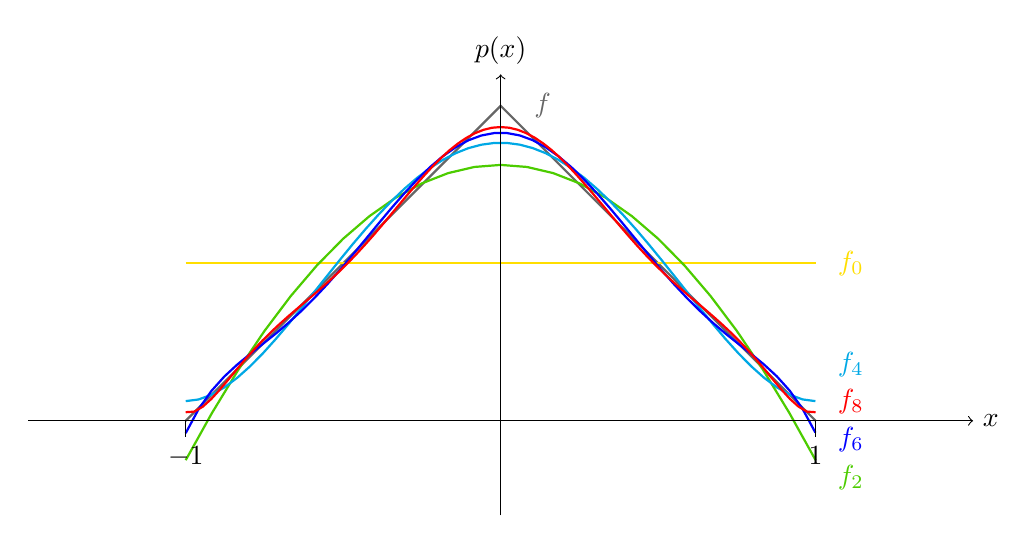
\begin{tikzpicture}[domain=-1:1, scale=4, samples=25]
      \def\fA#1{1}
      \def\fB#1{(#1)}
      \def\fC#1{(abs((#1)^2)-1/3)}
      \def\fD#1{((#1)^3-3/5*(#1))}
      \def\fE#1{(abs((#1)^4)-6/7*abs((#1)^2)+3/35)}
      \def\fF#1{((#1)^5 - 10/9*(#1)^3+5/21*(#1))}
      \def\fG#1{(abs((#1)^6)-15/11*abs((#1)^4)+5/11*abs((#1)^2)-5/231)}
      \def\fH#1{((429*(#1)^7 - 693*(#1)^5 + 315*(#1)^3 - 35*(#1))/429)}
      \def\fI#1{((6435*abs((#1)^8)-12012*abs((#1)^6)+6930*abs((#1)^4)-1260*abs((#1)^2)+35)/6435)}
      \definecolor{my-blue}{rgb}{0,0.66,0.9}
      \definecolor{my-yellow}{rgb}{1.00,0.87,0.00}
      \definecolor{my-gray}{rgb}{0.4,0.4,0.4}
      \definecolor{my-green}{rgb}{0.3,0.8,0}
      \definecolor{my-orange}{rgb}{1,0.5,0}
      \draw[thick,color=my-gray] (-1,0) -- (0,1) -- (1,0);
      \path[color=my-gray] (0,1) node[right=2ex] {$f$};
      \draw[thick,color=my-yellow] plot (\x,0.5*\fA{\x}) (1,0.5) node[right=1ex] {$f_0$};
      \draw[thick,color=my-green] plot (\x,{0.5*\fA{\x} - 0.9375*\fC{\x}}) (1,-0.18) node[right=1ex] {$f_2$};
      \draw[thick,color=my-blue,samples=50] plot (\x,{0.5*\fA{\x} - 0.9375*\fC{\x} + 0.8203125*\fE{\x}}) (1,0.18) node[right=1ex] {$f_4$};
      \draw[thick,color=blue,samples=50] plot (\x,{0.5*\fA{\x} - 0.9375*\fC{\x} + 0.8203125*\fE{\x} -1.46630859375*\fG{\x}}) (1,-0.06) node[right=1ex] {$f_6$};
      \draw[thick,color=red,samples=75] plot (\x,{0.5*\fA{\x} - 0.9375*\fC{\x} + 0.8203125*\fE{\x} -1.46630859375*\fG{\x}+3.338470458984375*\fI{\x}}) (1,0.06) node[right=1ex] {$f_8$};
      \draw[->] (-1.5,0) -- (1.5,0) node[right] {$x$};
      \draw[->] (0,-0.3) -- (0,1.1) node[above] {$p(x)$};
      \draw (1,0) -- (1,-0.05) node[below] {$1$};
      \draw (-1,0) -- (-1,-0.05) node[below] {$-1$};
    \end{tikzpicture}
  \end{center}
\end{solution}


% ======================================================================
% CONTINUE HERE...

\void{

% ----------------------------------------------------------------------
% Legendre 2

\begin{center}
  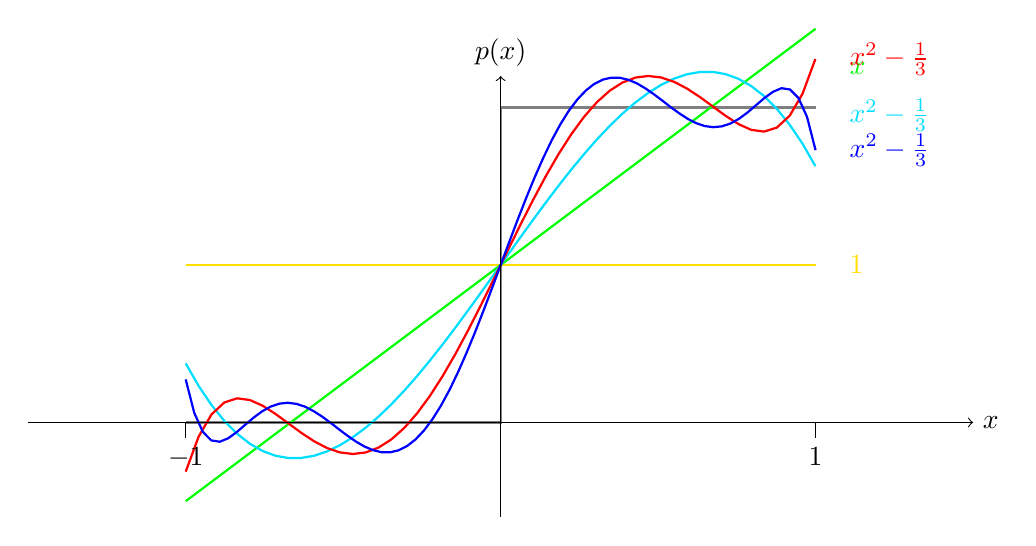
\begin{tikzpicture}[domain=-1:1, scale=4, samples=25]
    \def\fA#1{1}
    \def\fB#1{(#1)}
    \def\fC#1{(abs((#1)^2)-1/3)}
    \def\fD#1{((#1)^3-3/5*(#1))}
    \def\fE#1{(abs((#1)^4)-6/7*abs((#1)^2)+3/35)}
    \def\fF#1{((#1)^5 - 10/9*(#1)^3+5/21*(#1))}
    \def\fG#1{(abs((#1)^6)-15/11*abs((#1)^4)+5/11*abs((#1)^2)-5/231)}
    \def\fH#1{((429*(#1)^7 - 693*(#1)^5 + 315*(#1)^3 - 35*(#1))/429)}
    \def\fI#1{((6435*abs((#1)^8)-12012*abs((#1)^6)+6930*abs((#1)^4)-1260*abs((#1)^2)+35)/6435)}
    \definecolor{my-blue}{rgb}{0,0.87,1.00}
    \definecolor{my-yellow}{rgb}{1.00,0.87,0.00}
    \draw[thick,color=gray] (-1,0) -- (0,0) -- (0,1) -- (1,1);
    \draw[thick,color=my-yellow] plot (\x,0.5*\fA{\x}) node[right=2ex] {$1$};
    \draw[thick,color=green]     plot (\x,{0.5*\fA{\x} + 0.75*\fB{\x}}) node[below right=2ex] {$x$};
    \draw[thick,color=my-blue,samples=50]   plot (\x,{0.5*\fA{\x} + 0.75*\fB{\x} - 1.09375*\fD{\x}}) node[above right=2ex] {$x^2-\frac{1}{3}$};
    \draw[thick,color=red,samples=50]       plot (\x,{0.5*\fA{\x} + 0.75*\fB{\x} - 1.09375*\fD{\x} + 2.70703125*\fF{\x}}) node[right=2ex] {$x^2-\frac{1}{3}$};
    \draw[thick,color=blue,samples=75]      plot (\x,{0.5*\fA{\x} + 0.75*\fB{\x} - 1.09375*\fD{\x} + 2.70703125*\fF{\x} - 7.855224609375*\fH{\x}}) node[right=2ex] {$x^2-\frac{1}{3}$};
    \draw[->] (-1.5,0) -- (1.5,0) node[right] {$x$};
    \draw[->] (0,-0.3) -- (0,1.1) node[above] {$p(x)$};
    \draw (1,0) -- (1,-0.05) node[below] {$1$};
    \draw (-1,0) -- (-1,-0.05) node[below] {$-1$};
  \end{tikzpicture}
\end{center}

% ----------------------------------------------------------------------
% Legendre 3

\begin{center}
  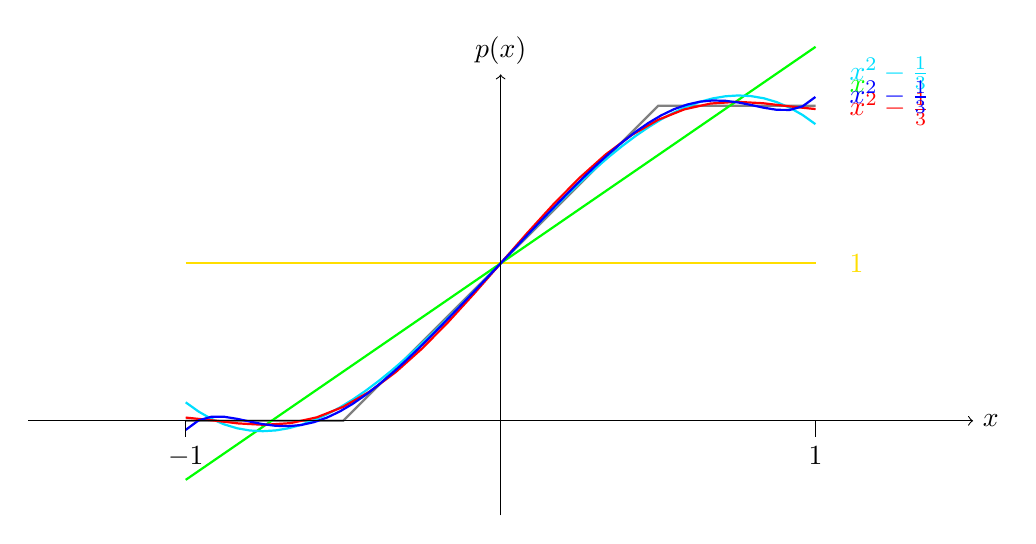
\begin{tikzpicture}[domain=-1:1, scale=4, samples=25]
    \def\fA#1{1}
    \def\fB#1{(#1)}
    \def\fC#1{(abs((#1)^2)-1/3)}
    \def\fD#1{((#1)^3-3/5*(#1))}
    \def\fE#1{(abs((#1)^4)-6/7*abs((#1)^2)+3/35)}
    \def\fF#1{((#1)^5 - 10/9*(#1)^3+5/21*(#1))}
    \def\fG#1{(abs((#1)^6)-15/11*abs((#1)^4)+5/11*abs((#1)^2)-5/231)}
    \def\fH#1{((429*(#1)^7 - 693*(#1)^5 + 315*(#1)^3 - 35*(#1))/429)}
    \def\fI#1{((6435*abs((#1)^8)-12012*abs((#1)^6)+6930*abs((#1)^4)-1260*abs((#1)^2)+35)/6435)}
    \definecolor{my-blue}{rgb}{0,0.87,1.00}
    \definecolor{my-yellow}{rgb}{1.00,0.87,0.00}
    \draw[thick,color=gray] (-1,0) -- (-0.5,0) -- (0.5,1) -- (1,1);
    \draw[thick,color=my-yellow] plot (\x,0.5*\fA{\x}) node[right=2ex] {$1$};
    \draw[thick,color=green]     plot (\x,{0.5*\fA{\x} + 0.6875*\fB{\x}}) node[below right=2ex] {$x$};
    \draw[thick,color=my-blue,samples=50]   plot (\x,{0.5*\fA{\x} + 0.6875*\fB{\x} - 0.615234375*\fD{\x}}) node[above right=2ex] {$x^2-\frac{1}{3}$};
    \draw[thick,color=red]       plot (\x,{0.5*\fA{\x} + 0.6875*\fB{\x} - 0.615234375*\fD{\x} + 0.38067626953125*\fF{\x}}) node[right=2ex] {$x^2-\frac{1}{3}$};
    \draw[thick,color=blue,samples=50]      plot (\x,{0.5*\fA{\x} + 0.6875*\fB{\x} - 0.615234375*\fD{\x} + 0.38067626953125*\fF{\x} + 1.0494089126587303*\fH{\x}}) node[right=2ex] {$x^2-\frac{1}{3}$};
    \draw[->] (-1.5,0) -- (1.5,0) node[right] {$x$};
    \draw[->] (0,-0.3) -- (0,1.1) node[above] {$p(x)$};
    \draw (1,0) -- (1,-0.05) node[below] {$1$};
    \draw (-1,0) -- (-1,-0.05) node[below] {$-1$};
  \end{tikzpicture}
\end{center}

% ----------------------------------------------------------------------
% Fourier 1

\begin{center}
  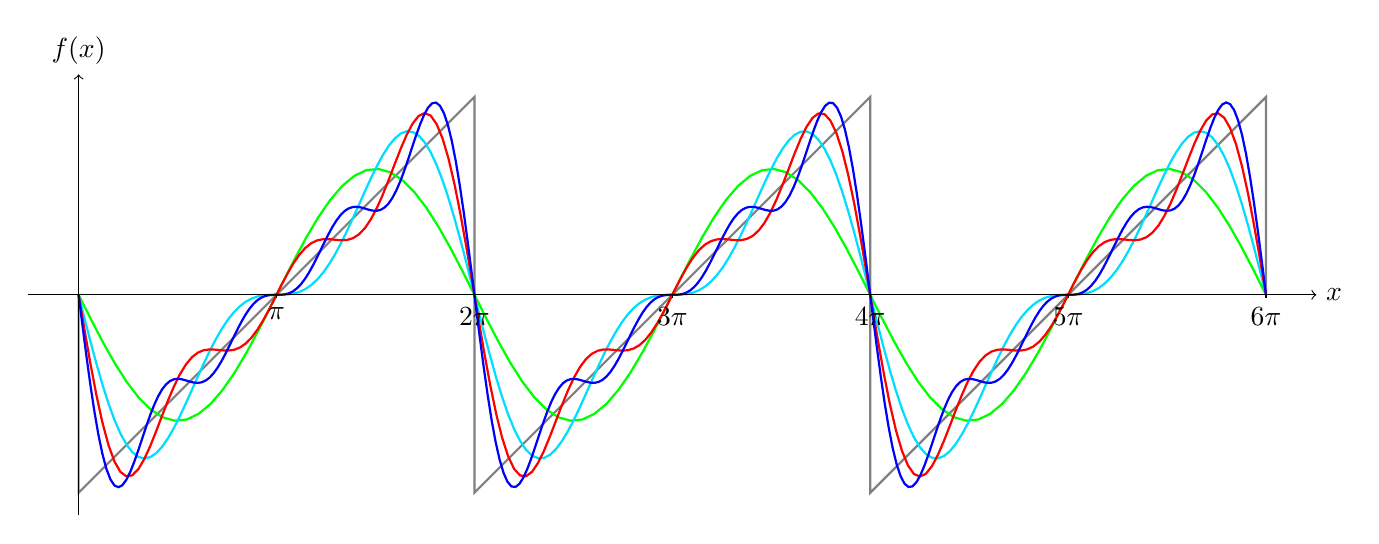
\begin{tikzpicture}[domain=0:6*pi, scale=0.8, samples=100]
    \def\fA#1{1}
    \def\fB#1{(sin((#1)/pi*180)}
    \def\fC#1{(cos((#1)/pi*180))}
    \def\fD#1{(sin(2*(#1)/pi*180))}
    \def\fE#1{(cos(2*(#1)/pi*180))}
    \def\fF#1{(sin(3*(#1)/pi*180))}
    \def\fG#1{(cos(3*(#1)/pi*180))}
    \def\fH#1{(sin(4*(#1)/pi*180))}
    \def\fI#1{(cos(4*(#1)/pi*180))}
    \definecolor{my-blue}{rgb}{0,0.87,1.00}
    \definecolor{my-yellow}{rgb}{1.00,0.87,0.00}
    \draw[thick,color=gray] (0,0) -- (0,-pi) -- (2*pi,pi) -- (2*pi,-pi) --
    (4*pi,pi) -- (4*pi,-pi) -- (6*pi, pi) -- (6*pi, 0);
    \draw[thick,color=green]   plot (\x,{((-2)*\fB{\x})}) node[below right=2ex] {};
    \draw[thick,color=my-blue,samples=200] plot (\x,{((-2)*\fB{\x})+((-1)*\fD{\x})}) node[above right=2ex] {};
    \draw[thick,color=red,samples=200]     plot (\x,{((-2)*\fB{\x})+((-1)*\fD{\x})+((-2/3)*\fF{\x})}) node[right=2ex] {};
    \draw[thick,color=blue,samples=300]    plot (\x,{((-2)*\fB{\x})+((-1)*\fD{\x})+((-2/3)*\fF{\x})+((-1/2)*\fH{\x})}) node[right=2ex] {};
    \draw[->] (-0.8,0) -- (6*pi+0.8,0) node[right] {$x$};
    \draw[->] (0,-3.5) -- (0,3.5) node[above] {$f(x)$};
    \draw (pi,0) -- (pi,-0.05) node[below] {$\pi$};
    \draw (2*pi,0) -- (2*pi,-0.05) node[below] {$2\pi$};
    \draw (3*pi,0) -- (3*pi,-0.05) node[below] {$3\pi$};
    \draw (4*pi,0) -- (4*pi,-0.05) node[below] {$4\pi$};
    \draw (5*pi,0) -- (5*pi,-0.05) node[below] {$5\pi$};
    \draw (6*pi,0) -- (6*pi,-0.05) node[below] {$6\pi$};
  \end{tikzpicture}
\end{center}

\begin{center}
  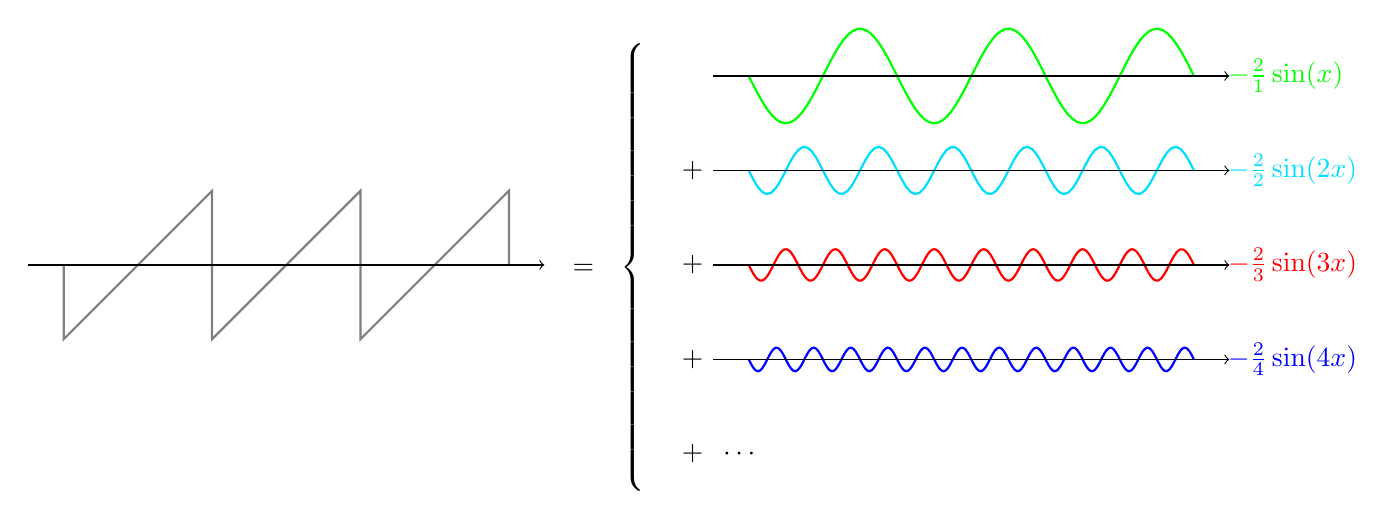
\begin{tikzpicture}[domain=0:6*pi, scale=0.3, samples=100]
    \def\fA#1{1}
    \def\fB#1{(sin((#1)/pi*180)}
    \def\fC#1{(cos((#1)/pi*180))}
    \def\fD#1{(sin(2*(#1)/pi*180))}
    \def\fE#1{(cos(2*(#1)/pi*180))}
    \def\fF#1{(sin(3*(#1)/pi*180))}
    \def\fG#1{(cos(3*(#1)/pi*180))}
    \def\fH#1{(sin(4*(#1)/pi*180))}
    \def\fI#1{(cos(4*(#1)/pi*180))}
    \definecolor{my-blue}{rgb}{0,0.87,1.00}
    \definecolor{my-yellow}{rgb}{1.00,0.87,0.00}
    \begin{scope}[yshift=-12cm,xshift=-29cm]
      \draw[thick,color=gray] (0,0) -- (0,-pi) -- (2*pi,pi) -- (2*pi,-pi) --
      (4*pi,pi) -- (4*pi,-pi) -- (6*pi, pi) -- (6*pi, 0);
      \draw[->] (-1.5,0) -- (6*pi+1.5,0)
      node[right]{$~~=~~\left\{\rule{0mm}{3cm}\right.$};
    \end{scope}
    \begin{scope}[yshift=-4cm]
      \draw[thick,color=green]   plot (\x,{((-2)*\fB{\x})}) node[right=2ex] {$-\frac{2}{1}\sin(x)$};
      \draw[->] (-1.5,0) -- (6*pi+1.5,0);
    \end{scope}
    \begin{scope}[yshift=-8cm]
      \draw[thick,color=my-blue] plot (\x,{((-1)*\fD{\x})}) node[right=2ex] {$-\frac{2}{2}\sin(2x)$};
      \draw[->] (-1.5,0) node[left]{$+$} -- (6*pi+1.5,0);
    \end{scope}
    \begin{scope}[yshift=-12cm]
      \draw[thick,color=red,samples=200]     plot (\x,{((-2/3)*\fF{\x})}) node[right=2ex] {$-\frac{2}{3}\sin(3x)$};
      \draw[->] (-1.5,0) node[left]{$+$} -- (6*pi+1.5,0);
    \end{scope}
    \begin{scope}[yshift=-16cm]
      \draw[thick,color=blue,samples=200]    plot (\x,{((-1/2)*\fH{\x})}) node[right=2ex] {$-\frac{2}{4}\sin(4x)$};
      \draw[->] (-1.5,0) node[left]{$+$} -- (6*pi+1.5,0);
    \end{scope}
    \begin{scope}[yshift=-20cm]
      \path (-1.5,0) node[left]{$+$} node[right]{$\cdots$};
    \end{scope}
  \end{tikzpicture}
\end{center}

% ----------------------------------------------------------------------
% Fourier 2

\begin{center}
  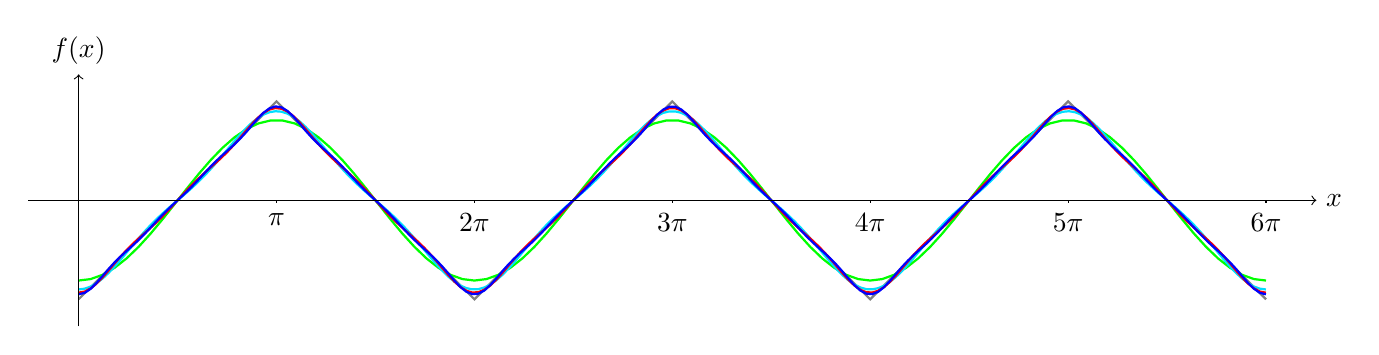
\begin{tikzpicture}[domain=0:6*pi, scale=0.8, samples=100]
    \def\fC#1{(cos((#1)/pi*180))}
    \def\fG#1{(cos(3*(#1)/pi*180))}
    \def\fK#1{(cos(5*(#1)/pi*180))}
    \def\fO#1{(cos(7*(#1)/pi*180))}
    \definecolor{my-blue}{rgb}{0,0.87,1.00}
    \definecolor{my-yellow}{rgb}{1.00,0.87,0.00}
    \draw[thick,color=gray] (0,-pi/2) -- (pi,pi/2) -- (2*pi,-pi/2) -- (3*pi,pi/2) --
    (4*pi,-pi/2) -- (5*pi,pi/2) -- (6*pi, -pi/2);
    \draw[thick,color=green]   plot (\x,{((-1.2732395447351623)*\fC{\x})}) node[below right=2ex] {};
    \draw[thick,color=my-blue,samples=200] plot (\x,{((-1.2732395447351623)*\fC{\x})+((-0.14147106052612904)*\fG{\x})}) node[above right=2ex] {};
    \draw[thick,color=red,samples=200]     plot (\x,{((-1.2732395447351623)*\fC{\x})+((-0.14147106052612904)*\fG{\x})+((-0.05092958178940641)*\fK{\x})}) node[above right=2ex] {};
    \draw[thick,color=blue,samples=200]    plot (\x,{((-1.2732395447351623)*\fC{\x})+((-0.14147106052612904)*\fG{\x})+((-0.05092958178940641)*\fK{\x})+((-0.025984480504798825)*\fO{\x})}) node[above right=2ex] {};
    \draw[->] (-0.8,0) -- (6*pi+0.8,0) node[right] {$x$};
    \draw[->] (0,-2) -- (0,2) node[above] {$f(x)$};
    \draw (pi,0) -- (pi,-0.05) node[below] {$\pi$};
    \draw (2*pi,0) -- (2*pi,-0.05) node[below] {$2\pi$};
    \draw (3*pi,0) -- (3*pi,-0.05) node[below] {$3\pi$};
    \draw (4*pi,0) -- (4*pi,-0.05) node[below] {$4\pi$};
    \draw (5*pi,0) -- (5*pi,-0.05) node[below] {$5\pi$};
    \draw (6*pi,0) -- (6*pi,-0.05) node[below] {$6\pi$};
  \end{tikzpicture}
\end{center}

\begin{center}
  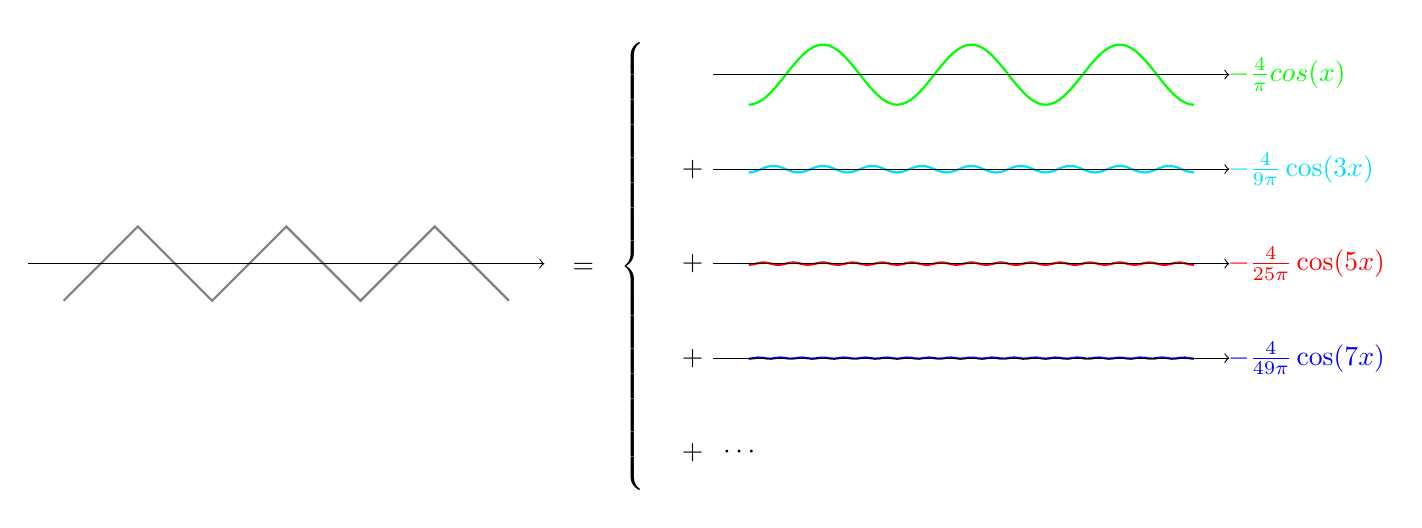
\begin{tikzpicture}[domain=0:6*pi, scale=0.3, samples=100]
    \def\fC#1{(cos((#1)/pi*180))}
    \def\fG#1{(cos(3*(#1)/pi*180))}
    \def\fK#1{(cos(5*(#1)/pi*180))}
    \def\fO#1{(cos(7*(#1)/pi*180))}
    \definecolor{my-blue}{rgb}{0,0.87,1.00}
    \definecolor{my-yellow}{rgb}{1.00,0.87,0.00}
    \begin{scope}[yshift=-12cm,xshift=-29cm]
      \draw[thick,color=gray] (0,-pi/2) -- (pi,pi/2) -- (2*pi,-pi/2) -- (3*pi,pi/2) --
      (4*pi,-pi/2) -- (5*pi,pi/2) -- (6*pi, -pi/2);
      \draw[->] (-1.5,0) -- (6*pi+1.5,0)
      node[right]{$~~=~~\left\{\rule{0mm}{3cm}\right.$};
    \end{scope}
    \begin{scope}[yshift=-4cm]
      \draw[thick,color=green]   plot (\x,{((-1.2732395447351623)*\fC{\x})}) (6*pi,0) node[right=2ex] {$-\frac{4}{\pi}cos(x)$};
      \draw[->] (-1.5,0) -- (6*pi+1.5,0);
    \end{scope}
    \begin{scope}[yshift=-8cm]
      \draw[thick,color=my-blue] plot (\x,{((-0.14147106052612904)*\fG{\x})}) (6*pi,0) node[right=2ex] {$-\frac{4}{9\pi}\cos(3x)$};
      \draw[->] (-1.5,0) node[left]{$+$} -- (6*pi+1.5,0);
    \end{scope}
    \begin{scope}[yshift=-12cm]
      \draw[thick,color=red]     plot (\x,{((-0.05092958178940641)*\fK{\x})}) (6*pi,0) node[right=2ex] {$-\frac{4}{25\pi}\cos(5x)$};
      \draw[->] (-1.5,0) node[left]{$+$} -- (6*pi+1.5,0);
    \end{scope}
    \begin{scope}[yshift=-16cm]
      \draw[thick,color=blue]    plot (\x,{((-0.025984480504798825)*\fO{\x})}) (6*pi,0) node[right=2ex] {$-\frac{4}{49\pi}\cos(7x)$};
      \draw[->] (-1.5,0) node[left]{$+$} -- (6*pi+1.5,0);
    \end{scope}
    \begin{scope}[yshift=-20cm]
      \path (-1.5,0) node[left]{$+$} node[right]{$\cdots$};
    \end{scope}
  \end{tikzpicture}
\end{center}

% ----------------------------------------------------------------------
% Fourier 3

\begin{center}
  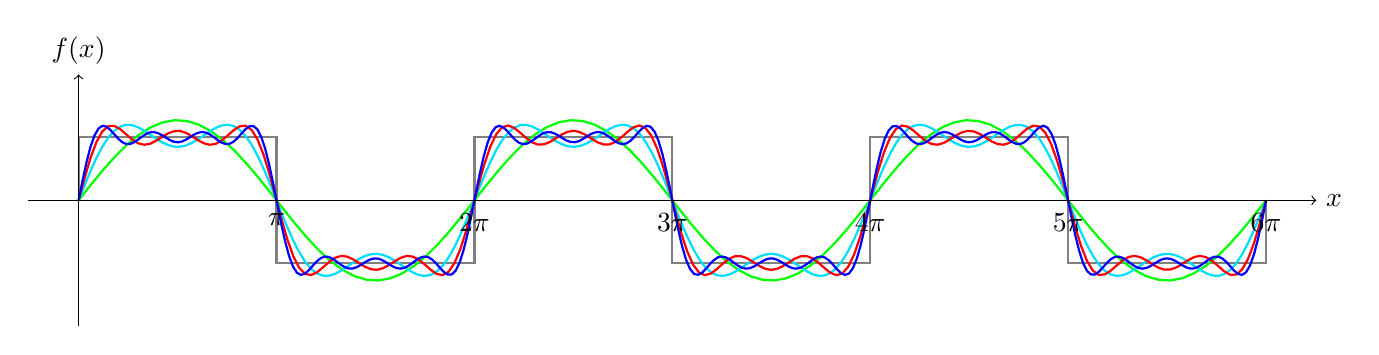
\begin{tikzpicture}[domain=0:6*pi, scale=0.8, samples=100]
    \def\fB#1{(sin((#1)/pi*180))}
    \def\fF#1{(sin(3*(#1)/pi*180))}
    \def\fJ#1{(sin(5*(#1)/pi*180))}
    \def\fN#1{(sin(7*(#1)/pi*180))}
    \definecolor{my-blue}{rgb}{0,0.87,1.00}
    \definecolor{my-yellow}{rgb}{1.00,0.87,0.00}
    \draw[thick,color=gray] (0,0) -- (0,1) -- (pi,1) -- (pi,-1) --
    (2*pi,-1) -- (2*pi,1) --
    (3*pi,1) -- (3*pi,-1) --
    (4*pi,-1) -- (4*pi,1) --
    (5*pi,1) -- (5*pi,-1) --
    (6*pi,-1) -- (6*pi,0);
    \draw[thick,color=green]   plot (\x,{((1.2732395447351623)*\fB{\x})}) node[below right=2ex] {};
    \draw[thick,color=my-blue,samples=200] plot (\x,{((1.2732395447351623)*\fB{\x})+((0.4244131815783881)*\fF{\x})}) node[above right=2ex] {};
    \draw[thick,color=red,samples=200]     plot (\x,{((1.2732395447351623)*\fB{\x})+((0.4244131815783881)*\fF{\x})+((0.25464790894703326)*\fJ{\x})}) node[above right=2ex] {};
    \draw[thick,color=blue,samples=300]    plot (\x,{((1.2732395447351623)*\fB{\x})+((0.4244131815783881)*\fF{\x})+((0.25464790894703326)*\fJ{\x})+((0.18189136353359486)*\fN{\x})}) node[above right=2ex] {};
    \draw[->] (-0.8,0) -- (6*pi+0.8,0) node[right] {$x$};
    \draw[->] (0,-2) -- (0,2) node[above] {$f(x)$};
    \draw (pi,0) -- (pi,-0.05) node[below] {$\pi$};
    \draw (2*pi,0) -- (2*pi,-0.05) node[below] {$2\pi$};
    \draw (3*pi,0) -- (3*pi,-0.05) node[below] {$3\pi$};
    \draw (4*pi,0) -- (4*pi,-0.05) node[below] {$4\pi$};
    \draw (5*pi,0) -- (5*pi,-0.05) node[below] {$5\pi$};
    \draw (6*pi,0) -- (6*pi,-0.05) node[below] {$6\pi$};
  \end{tikzpicture}
\end{center}

\begin{center}
  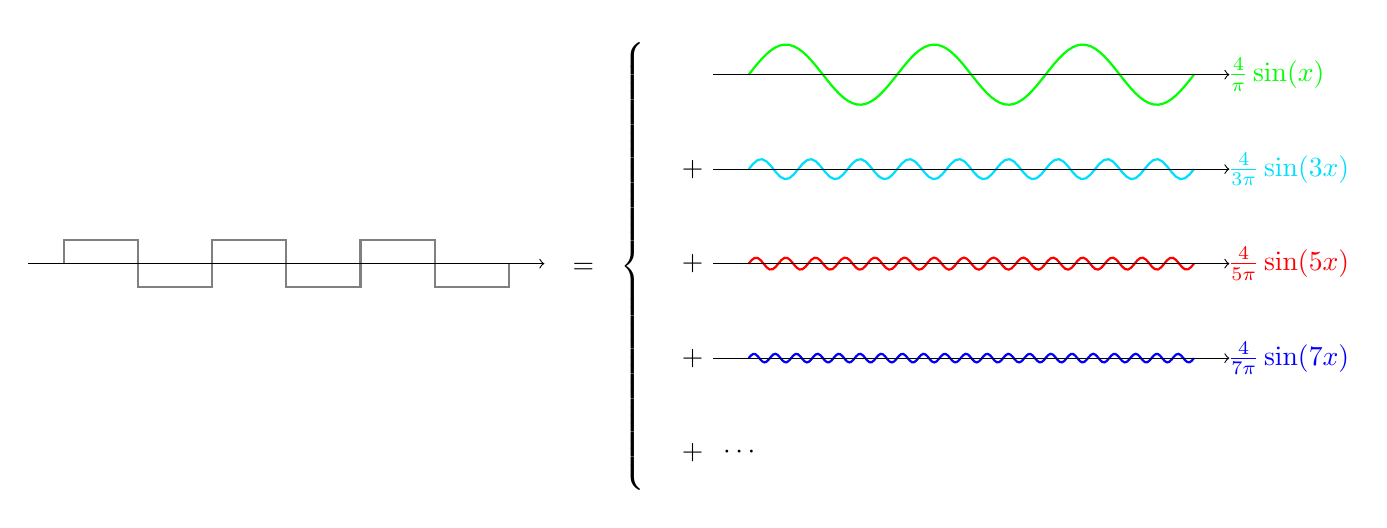
\begin{tikzpicture}[domain=0:6*pi, scale=0.3, samples=100]
    \def\fB#1{(sin((#1)/pi*180))}
    \def\fF#1{(sin(3*(#1)/pi*180))}
    \def\fJ#1{(sin(5*(#1)/pi*180))}
    \def\fN#1{(sin(7*(#1)/pi*180))}
    \definecolor{my-blue}{rgb}{0,0.87,1.00}
    \definecolor{my-yellow}{rgb}{1.00,0.87,0.00}
    \begin{scope}[yshift=-12cm,xshift=-29cm]
      \draw[thick,color=gray] (0,0) -- (0,1) -- (pi,1) -- (pi,-1) --
      (2*pi,-1) -- (2*pi,1) --
      (3*pi,1) -- (3*pi,-1) --
      (4*pi,-1) -- (4*pi,1) --
      (5*pi,1) -- (5*pi,-1) --
      (6*pi,-1) -- (6*pi,0);
      \draw[->] (-1.5,0) -- (6*pi+1.5,0)
      node[right]{$~~=~~\left\{\rule{0mm}{3cm}\right.$};
    \end{scope}
    \begin{scope}[yshift=-4cm]
      \draw[thick,color=green]   plot (\x,{((1.2732395447351623)*\fB{\x})}) node[right=2ex] {$\frac{4}{\pi}\sin(x)$};
      \draw[->] (-1.5,0) -- (6*pi+1.5,0);
    \end{scope}
    \begin{scope}[yshift=-8cm]
      \draw[thick,color=my-blue] plot (\x,{((0.4244131815783881)*\fF{\x})}) node[right=2ex] {$\frac{4}{3\pi}\sin(3x)$};
      \draw[->] (-1.5,0) node[left]{$+$} -- (6*pi+1.5,0);
    \end{scope}
    \begin{scope}[yshift=-12cm]
      \draw[thick,color=red,samples=150]     plot (\x,{((0.25464790894703326)*\fJ{\x})}) node[right=2ex] {$\frac{4}{5\pi}\sin(5x)$};
      \draw[->] (-1.5,0) node[left]{$+$} -- (6*pi+1.5,0);
    \end{scope}
    \begin{scope}[yshift=-16cm]
      \draw[thick,color=blue,samples=200]    plot (\x,{((0.18189136353359486)*\fN{\x})}) node[right=2ex] {$\frac{4}{7\pi}\sin(7x)$};
      \draw[->] (-1.5,0) node[left]{$+$} -- (6*pi+1.5,0);
    \end{scope}
    \begin{scope}[yshift=-20cm]
      \path (-1.5,0) node[left]{$+$} node[right]{$\cdots$};
    \end{scope}
  \end{tikzpicture}
\end{center}
}
